\section{Exercise 10}
\subsection{}
\begin{itemize}
  \item [a] ($\gamma$ = 0.2, n = 0, r = 0)
  \item [b] ($\gamma$ = 0.5, n = 0.1, r = -1)
  \item [c] ($\gamma$ = 0.5, n = 0, r = 0)
  \item [d] ($\gamma$ = 0.5, n = 0.25, r = 0)
  \item [e] ($\gamma$ = 0, n = 0, r = 0)
\end{itemize}

\subsection{}
For this exercise we have plotted formulae to compute the value / score of different path options. We have chosen X axis to represent the discount and Y axis to represent value / score of the given path option. \\ \smallskip
Legend for the following figures:
\begin{itemize}
  \item [\textbf{n}] Noise parameter
  \item [\textbf{l}] Living reward parameter
  \item [\textbf{Red line}] Prefer the close exit (+1), risking the cliff (-10)
  \item [\textbf{Blue line}] Prefer the distant exit (+10), risking the cliff (-10)
  \item [\textbf{Green line}] Prefer the distant exit (+10), avoiding the cliff (-10)
  \item [\textbf{Purple line}] Prefer the close exit (+1), but avoiding the cliff (-10)
\end{itemize}


\subsubsection{a}
Because noise is 0 this path is considered safe. Therefore agent would go along the bridge. If discount is low enough the shorter path will be preferred. This preference is amplified if living reward is negative. \\ 
We have chosen for for discount of 0.2 since that allows other parameters be unchanged. See \Fgcite{fig:e101} the red line.

\begin{figure}[H]
\caption{}
\centering
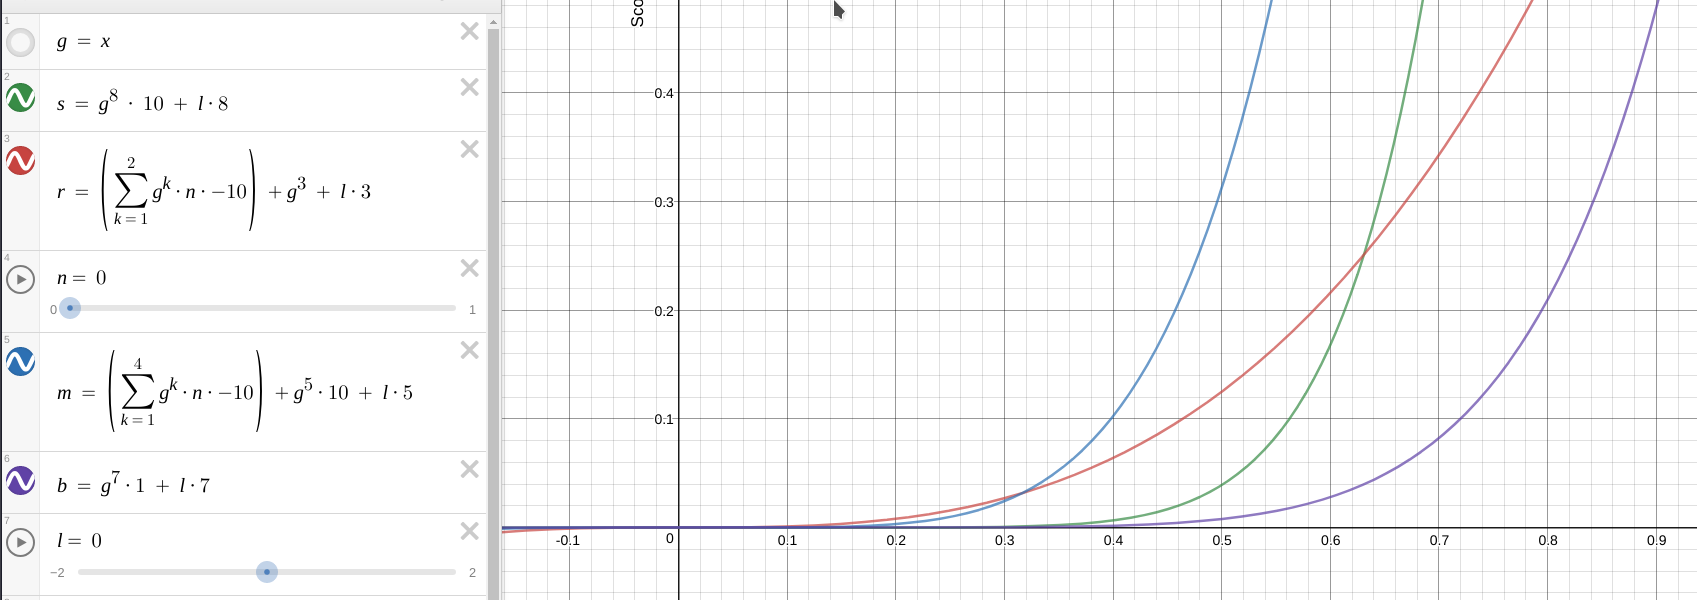
\includegraphics[width=12cm]{plot_10_1}
\label{fig:e101}
\end{figure}

\subsubsection{b}
Here we make living reward negative to discover long routes. Along with this we make noise big to discourage risk. With this we see that purple line has a higher value then other paths with discount of 0.5, noise of 0.1 and living reward of -1.

\subsubsection{c}
Here we set noise to 0 to remove any risks and we make long term reward (discount) tempting enough to pick the longest path along the bridge. We can see with noise and living reward set to 0 that the blue line has the higher score than other paths at discount of 0.5. See \Fgcite{fig:e103} the blue line.

\begin{figure}[H]
\caption{}
\centering
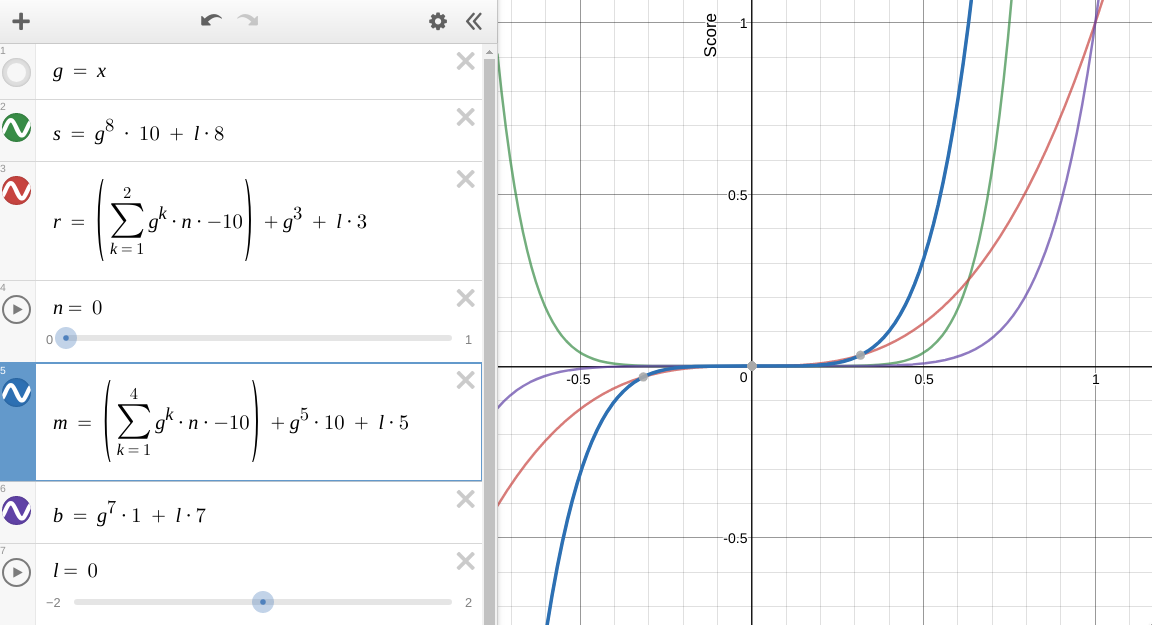
\includegraphics[width=12cm]{plot_10_3}
\label{fig:e103}
\end{figure}

\subsubsection{d}
Here we set noise high enough to discourage risk and pick the right discount to encourage long term reward. At discount of 0.5 green line has the highest value. See \Fgcite{fig:e104} the green line.

\begin{figure}[H]
\caption{}
\centering
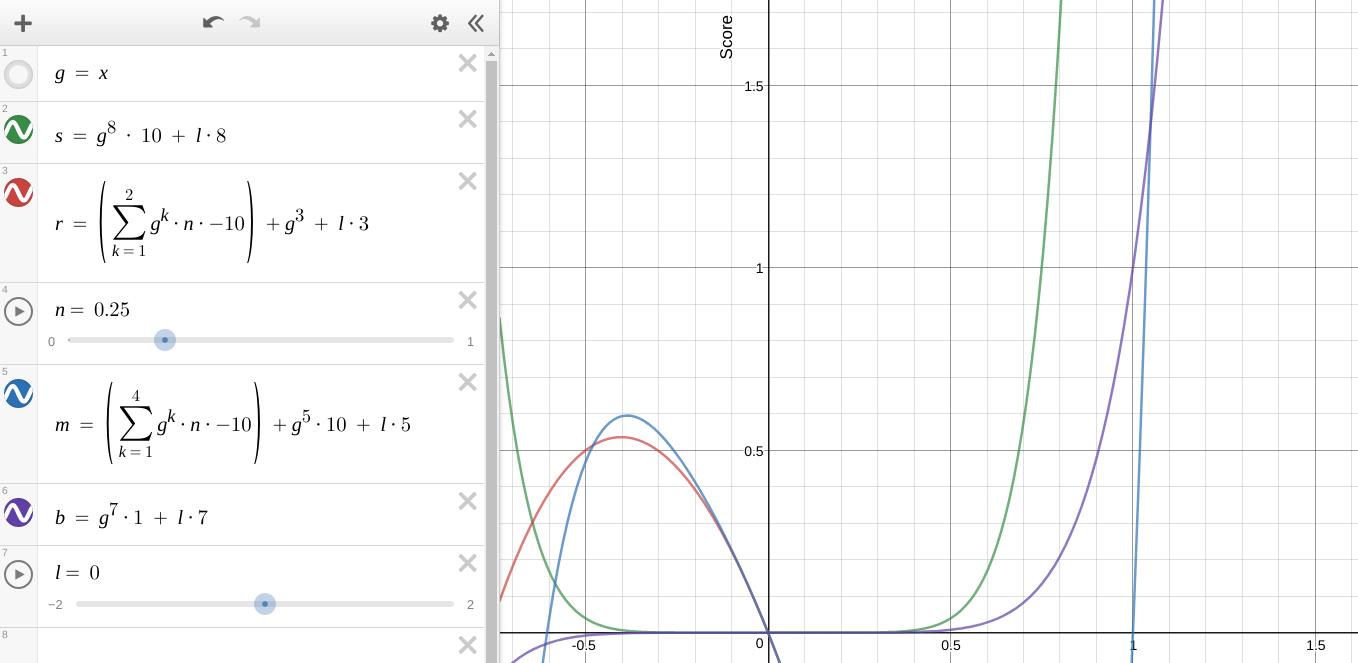
\includegraphics[width=12cm]{plot_10_4}
\label{fig:e104}
\end{figure}

\subsubsection{e}
Here we put everything at zero. Because reward is getting multiplied by gamma and gamma is set to 0, every Q-value will also be zero and thus the episode would never terminate.